\documentclass[12pt,a4paper]{article}

\usepackage{amsmath}
\usepackage{graphicx}
\usepackage{float}
\usepackage{geometry}
\usepackage{booktabs}
\usepackage{listings}
\usepackage{xcolor}
\begin{document}
    

\begin{minipage}{0.6\textwidth}

\includegraphics[width=0.75\textwidth]{IIITB-COMET-Logo.png}
\end{minipage}
\begin{minipage}{0.38\textwidth}
\begin{flushright}
\textbf{DARSI VAMSI}
\newline
\textbf{COMET FWC 071}
\end{flushright}
\end{minipage}

\section*{\textbf{Implementation of a Boolean Expression Using Arduino UNO, SN74LS47N Decoder and Seven Segment Display}}






To implement the Boolean expression obtained from the given logic circuit using Arduino UNO, SN74LS47N BCD-to-Seven Segment Decoder and a Common Anode Seven Segment Display.

\section*{Apparatus Required}

\begin{itemize}
\item Arduino UNO
\item SN74LS47N BCD-to-Seven Segment Decoder
\item Common Anode Seven Segment Display
\item Breadboard
\item Connecting Wires
\item 220$\Omega$ Resistors
\item USB Cable
\end{itemize}

\section*{Logic Diagram}

\begin{figure}[H]
\centering
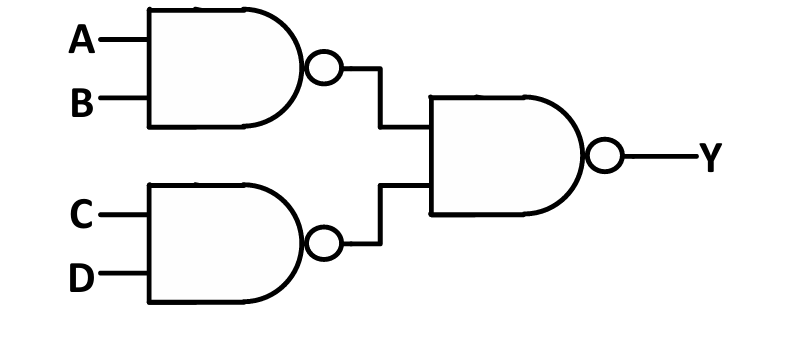
\includegraphics[width=0.65\textwidth,height=2 cm]{figure.png}
\caption{Given Logic Circuit}
\label{fig:logic}
\end{figure}

\begin{equation}
Y = AB + CD
\end{equation}

The Boolean expression is evaluated by the Arduino UNO. The resulting output is sent as BCD data to the SN74LS47N decoder, which drives a Common Anode Seven Segment Display.

\section*{Truth Table}

\begin{table}[H]
\centering
\caption{Truth Table of the Boolean Expression}
\begin{tabular}{|c|c|c|c|c|}
\hline
A & B & C & D & Y = AB + CD \\
\hline
0 & 0 & 0 & 0 & 0 \\
\hline
1 & 1 & 0 & 0 & 1 \\
\hline
0 & 1 & 0 & 1 & 0 \\
\hline
0 & 0 & 1 & 1 & 1 \\
\hline
\end{tabular}
\end{table}

\section*{Pin Connections}

\subsection*{Arduino UNO to SN74LS47N}

\begin{table}[H]
\centering
\caption{Arduino to Decoder Connections}
\begin{tabular}{|c|c|}
\hline
Arduino Pin & SN74LS47N Pin \
\hline
D9 & A (Pin 7) \\
\hline
D10 & B (Pin 1) \\
\hline
D11 & C (Pin 2) \\
\hline
D12 & D (Pin 6) \\
\hline
5V & VCC (Pin 16) \\
\hline
GND & GND (Pin 8) \\
\hline
\end{tabular}
\end{table}

\subsection*{SN74LS47N Control Pins}

\begin{table}[H]
\centering
\caption{Control Pin Connections}
\begin{tabular}{|c|c|}
\hline
SN74LS47N Pin & Connection \\
\hline
LT (Pin 3) & +5V \\
\hline
RBI (Pin 4) & +5V \\
\hline
BI/RBO (Pin 5) & +5V \\
\hline
\end{tabular}
\end{table}

\subsection*{SN74LS47N to Seven Segment Display}

\begin{table}[H]
\centering
\caption{Decoder to Display Connections}
\begin{tabular}{|c|c|}
\hline
SN74LS47N Output & Seven Segment Segment \\
\hline
a (Pin 13) & a \\
\hline
b (Pin 12) & b \\
\hline
c (Pin 11) & c \\
\hline
d (Pin 10) & d \\
\hline
e (Pin 9)  & e \\
\hline
f (Pin 15) & f \\
\hline
g (Pin 14) & g \\
\hline
\end{tabular}
\end{table}

\subsection*{Common Anode Connections}

\begin{table}[H]
\centering
\caption{Common Anode Display Connections}
\begin{tabular}{|c|c|}
\hline
Display Pin & Connection \\
\hline
Common Anode Pin 1 & +5V \\
\hline
Common Anode Pin 2 & +5V \\
\hline
\end{tabular}
\end{table}


\section*{Observations}

\begin{table}[H]
\centering
\caption{Experimental Verification}
\begin{tabular}{|c|c|c|c|c|}
\hline
A & B & C & D & Displayed Output \\
\hline
0 & 0 & 0 & 0 & 0 \\
\hline
1 & 1 & 0 & 0 & 1 \\
\hline
0 & 1 & 0 & 1 & 0 \\
\hline
0 & 0 & 1 & 1 & 1 \\
\hline
\end{tabular}
\end{table}

The output sequence observed on the seven segment display is

\begin{equation}
0 \rightarrow 1 \rightarrow 0 \rightarrow 1
\end{equation}

\section*{Result}

The Boolean expression

\begin{equation}
Y = AB + CD
\end{equation}

was successfully implemented using Arduino UNO, SN74LS47N BCD-to-Seven Segment Decoder and a Common Anode Seven Segment Display. The experimental results matched the expected truth table outputs. \newline
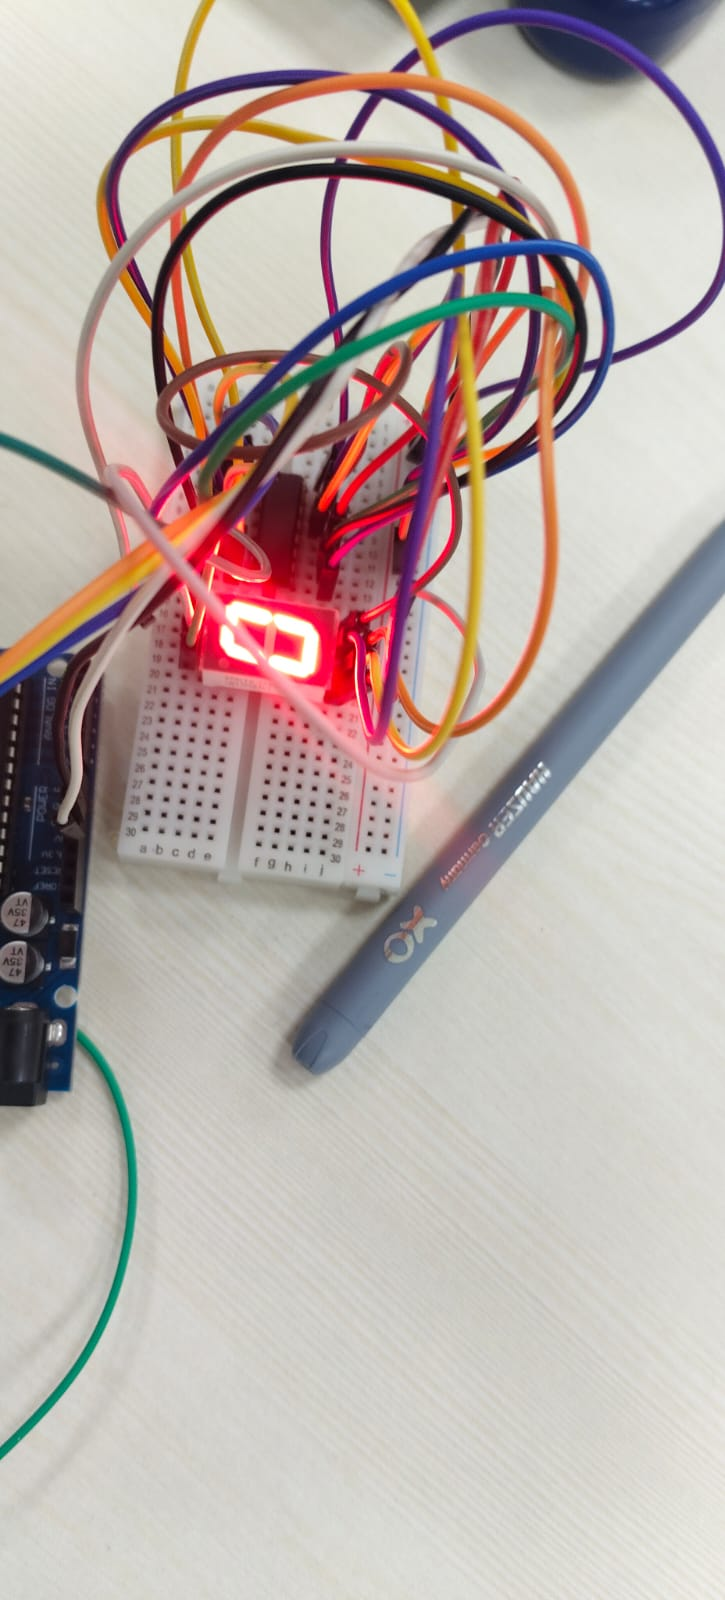
\includegraphics[width=0.75\textwidth ,height=7 cm]{Output_as zero.jpeg} \newline

\includegraphics[width=0.75\textwidth, height=7 cm]{output_as_1.jpeg} 
\end{document}
